\documentclass[10pt,a4paper]{beamer}

\usepackage[utf8]{inputenc}
\usepackage[russian]{babel}
\usepackage[OT1]{fontenc}
\usepackage{amsmath}
\usepackage{amsfonts}
\usepackage{amssymb}
\usepackage{makeidx}
\usepackage{graphicx}
\usepackage{xcolor}
\usepackage{multirow}
\usepackage{framed}
\definecolor{shadecolor}{cmyk}{0,0,0,1}

\titlegraphic{
   
\includegraphics[width=4cm]{images/sfera.jpg}
}

\author{Николай Анохин \and Михаил Фирулик}
\title{Введение в Data Science \\ Занятие 6. Кластеризация}

\beamertemplatenavigationsymbolsempty

\begin{document}

\maketitle

\logo{
    
\includegraphics[width=4cm,keepaspectratio]{images/sfera.jpg}\hspace{0.45em}
}

% ============================================== %

\begin{frame}{План занятия}

\tableofcontents

\end{frame}

% ============================================== %

\section{Задача кластеризации}

% ============================================== %

\begin{frame}{Python-программисты (by Gilad Lotan)}

\begin{center}
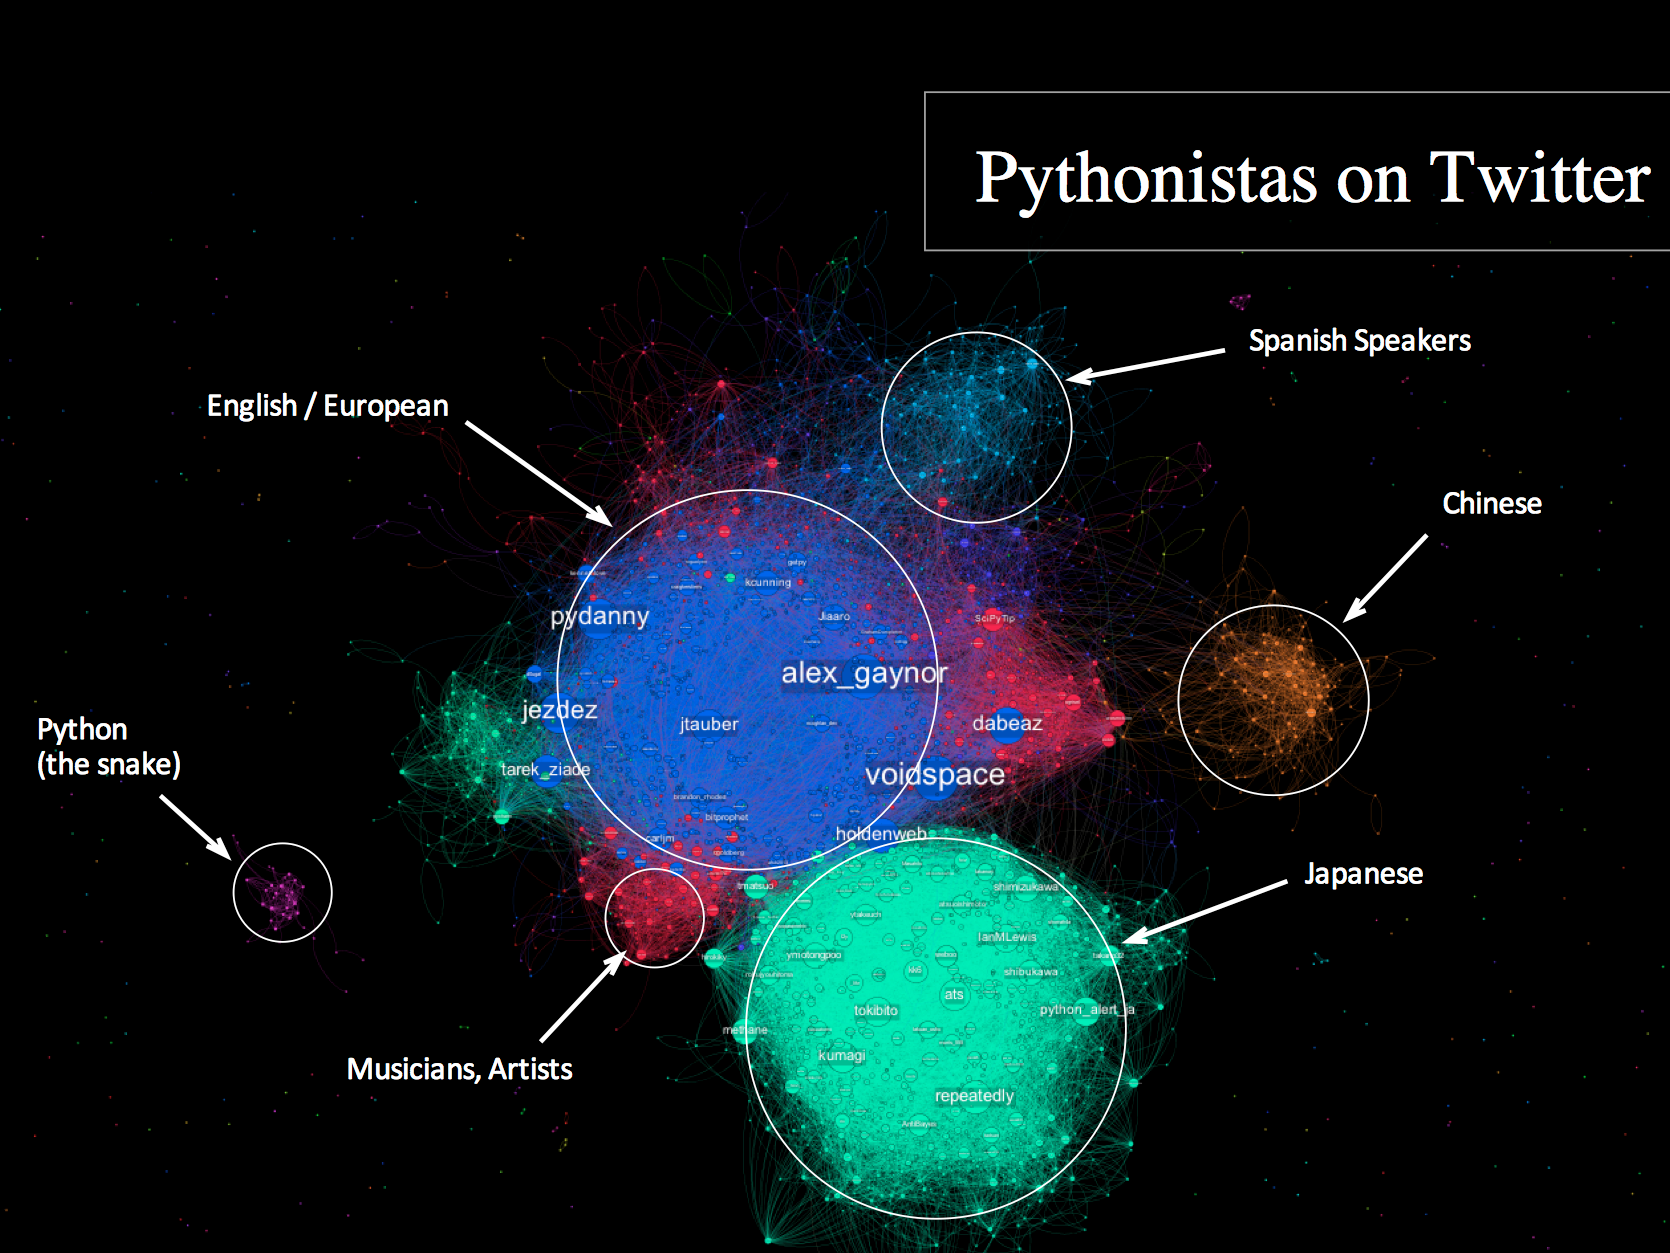
\includegraphics[scale=0.16]{images/python.png}
\end{center}

\end{frame}

% ============================================== %

\begin{frame}{Слова и топики}

\begin{center}
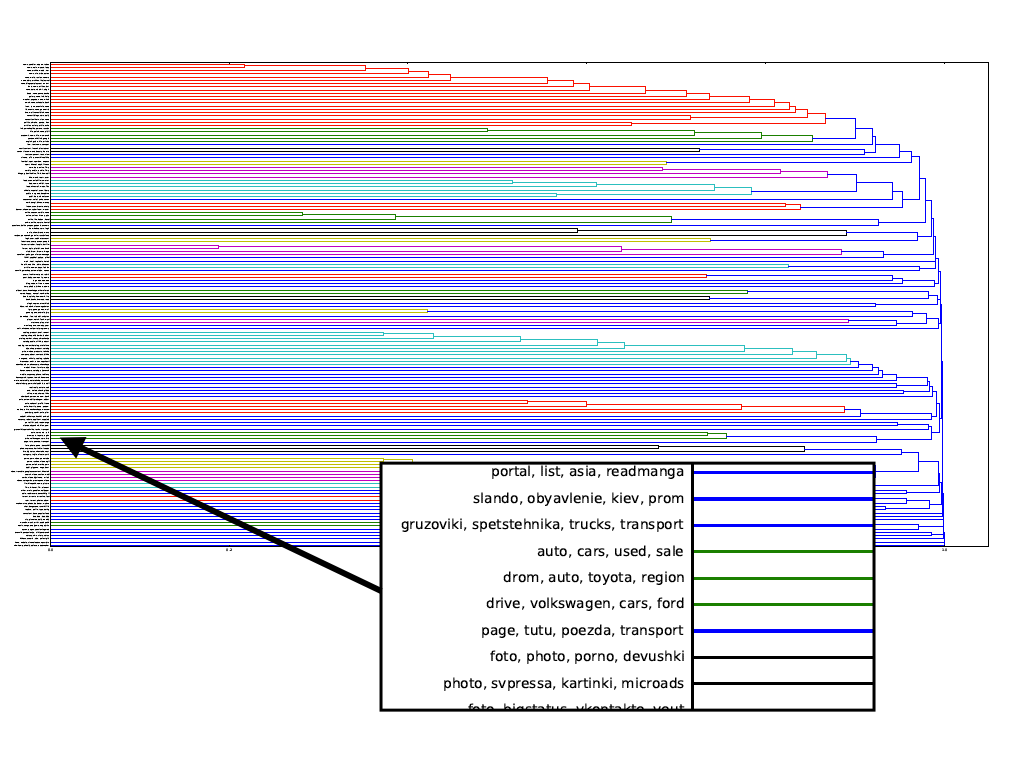
\includegraphics[scale=0.27]{images/hier.png}
\end{center}

\end{frame}

% ============================================== %

\begin{frame}{Интуиция}

\begin{exampleblock}{Кластерный анализ}
Разбиение множества обучающих объектов на непересекающиеся подмножества (кластеры) с использованием некоторой функции расстояния между объектами так, чтобы любые два объекта, лежащие в одном кластере были схожи, а любые два объекта, лежащие в разных кластерах существенно различались.
\end{exampleblock}

\end{frame}

% ============================================== %

\begin{frame}{Зачем}

\begin{columns}[T]
    \begin{column}{.55\textwidth}
    \begin{itemize}
	\item расширение обучающей выборки
	\item ручная разметка объектов
	\item конструирование признаков 
	\end{itemize}
    \end{column}
       
    \begin{column}{.45\textwidth}
    \begin{itemize}
	\item суммаризация данных
	\item визуализация данных
	\end{itemize}
	\end{column}
  \end{columns}

    \begin{center}
    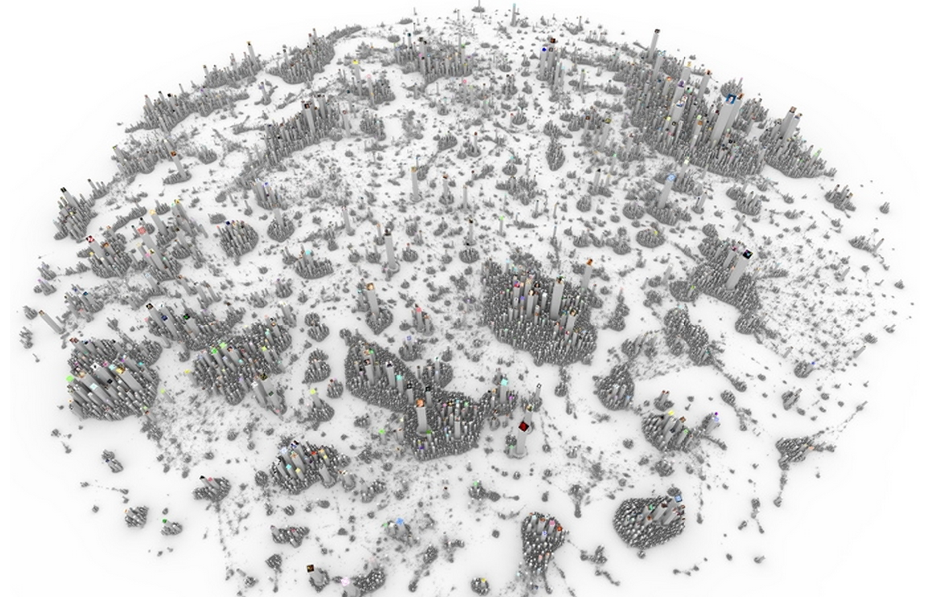
\includegraphics[scale=0.26]{images/sover.png}
    \end{center}

\end{frame}

% ============================================== %

\begin{frame}{Формально}

{\bf Дано:}
\begin{itemize}
\item Обучающая выборка $(\mathbf x_1, \ldots, \mathbf x_N)$, где $\mathbf{x}_j$ -- объект, принадлежащий некоторому множеству $\mathbf{X}$
\item На $\mathbf{X}$ определена функция расстояния (схожести)
\end{itemize}

\vspace{1em}
{\bf Найти:}
Разбиение $f: \mathbf{X} \rightarrow C$, где $C = \{1, \ldots, K\}$ -- множество идентификаторов  $K$ кластеров.

\end{frame}

% ============================================== %

\section{Функции расстояния}

% ============================================== %

\begin{frame}{Функция расстояния}

\begin{exampleblock}{Def}
Функция $d(\mathbf{x}, \mathbf{y}): \mathbf{X} \times \mathbf{X} \rightarrow R$ является функцией расстояния, определенной на пространстве $\mathbf{X}$ тогда и только тогда, когда $\forall \mathbf{x} \in \mathbf{X}, \; \forall \mathbf{y} \in \mathbf{X}, \; \forall \mathbf{z} \in \mathbf{X}$ выполнено:
\begin{enumerate}
\item $d(\mathbf{x}, \mathbf{y}) \geq 0$
\item $d(\mathbf{x}, \mathbf{y}) = 0 \Leftrightarrow \mathbf{x} = \mathbf{y}$
\item $d(\mathbf{x}, \mathbf{y}) = d(\mathbf{y}, \mathbf{x})$
\item $d(\mathbf{x}, \mathbf{y}) \leq d(\mathbf{x}, \mathbf{z}) + d(\mathbf{y}, \mathbf{z})$
\end{enumerate}
\end{exampleblock}

\end{frame}

% ============================================== %

\begin{frame}{Расстояния 1}

\begin{columns}[T]
    \begin{column}{.5\textwidth}
    \begin{itemize}
		\item Минковского
		\[
		d_r(\mathbf{x}, \mathbf{y}) = \left[ \sum_{j=1}^N |x_j - y_j|^r \right]^{\frac{1}{r}}
		\]
		\item Евклидово $r = 2$
		\[
		d_E(\mathbf{x}, \mathbf{y}) = d_2(\mathbf{x}, \mathbf{y})
		\]
		\item Манхэттэн $r = 1$
		\[
		d_M(\mathbf{x}, \mathbf{y}) = d_1(\mathbf{x}, \mathbf{y})
		\]
		\item $r=\infty$
		\[
		d_\infty(\mathbf{x}, \mathbf{y}) = \max_j |x_j - y_j|
		\]
	\end{itemize}
    \end{column}
       
    \begin{column}{.5\textwidth}
    \vspace{2em}
	\begin{center}
   		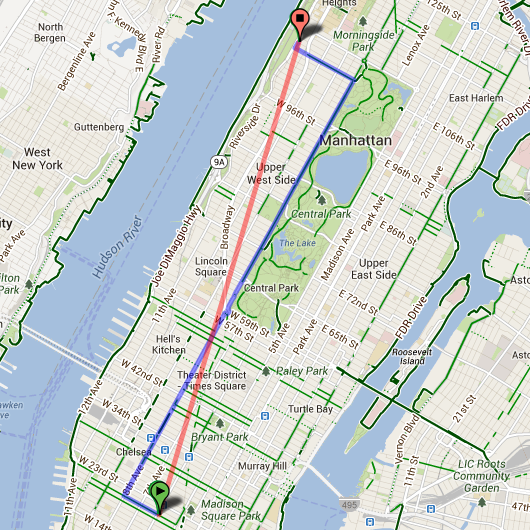
\includegraphics[scale=0.25]{images/manhattan.png}
    \end{center}
    \end{column}
  \end{columns}

\end{frame}

% ============================================== %

\begin{frame}{Проблема}

Функции расстояния чувствительны к преобразоаниям данных

\vspace{1em}
Решение
\begin{itemize}
\item Преобразовать обучающую выборку так, чтобы  признаки имели нулевое среднее и единичную дисперсию -- инвариантность к растяжению и сдвигу (stanartize)
\item Преобразовать обучающую выборку так, чтобы оси совпадали с главными компонентами матрицы ковариации -- инвариантность относительно поворотов (PCA)
\end{itemize}


\end{frame}

% ============================================== %

\begin{frame}{Расстояния 2}

\begin{columns}[T]

    \begin{column}{.4\textwidth}
    \vspace{5em}
	\begin{center}
   		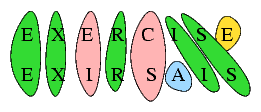
\includegraphics[scale=0.5]{images/edit.png}
    \end{center}
    \end{column}
       
    \begin{column}{.6\textwidth}
    \begin{itemize}
		\item Жаккар
		\[
		d_J(\mathbf{x}, \mathbf{y}) = 1 - \frac{|\mathbf{x} \cap \mathbf{y}|}{|\mathbf{x} \cup \mathbf{y}|}
		\]
		\item Косинус
		\[
		d_c(\mathbf{x}, \mathbf{y}) = \arccos \frac{\mathbf{x} \mathbf{y}}{\|\mathbf{x}\| \|\mathbf{y}\|}
		\]
		\item Правки \\
		{\it $d_e$ -- наименьшее количество удалений и вставок, приводящее $\mathbf{x}$ к $\mathbf{y}$.}
		\item Хэмминг \\
		{\it $d_H$ -- количество различных компонент в $\mathbf{x}$ и $\mathbf{y}$.}
	\end{itemize}
    
    \end{column}
  \end{columns}

\end{frame}

% ============================================== %

\begin{frame}{Проклятие размерности}

\begin{block}{Задача}
Даны два случайных вектора $\mathbf{x}$ и $\mathbf{y}$ в пространстве размерности $D$. Как зависит математическое ожидание косинус-расстояния между $\mathbf{x}$ и $\mathbf{y}$ от размерности $D$?
\end{block}

\[
d_c(\mathbf{x}, \mathbf{y}) = \arccos \frac{\sum_{j=1}^D x_j y_j}{\sum_{j=1}^D x_j^2 \sum_{j=1}^D y_j^2}
\]
Наблюдения:
\begin{itemize}
\item числитель стремится к нулю
\item знаменатель положительный
\end{itemize}
Вывод: $d_c(\mathbf{x}, \mathbf{y}) \rightarrow \frac \pi 2$.

\end{frame}

% ============================================== %

\section{Критерии качества кластеризации}

% ============================================== %

\begin{frame}{Выбор разбиения}

\begin{columns}[T]

    \begin{column}{.8\textwidth}
    \vspace{5em}
   \begin{block}{Идея}
	Определить критерий качества кластеризации $J$ и выбрать разбиение выборки на 				кластеры, которое которое соответствует оптимальному значению этого критерия.
	\end{block}
    \end{column}
       
    \begin{column}{.2\textwidth}
    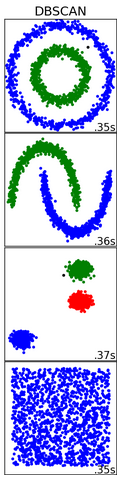
\includegraphics[scale=0.4]{images/dbscan.png}    
    \end{column}
  \end{columns}



\end{frame}

% ============================================== %

\begin{frame}{Квардатичная ошибка}

  \begin{columns}[T]
       
    \begin{column}{.5\textwidth}
    Среднее $k$-го кластера
	\[
		\mathbf{m}_k = \frac{1}{n_k} \sum_{\mathbf{x}_i \in C_k} \mathbf{x}_i
	\]
	Критерий
	\[
	J_E = \sum_{k=1}^K \sum_{\mathbf{x}_i \in C_k} \| \mathbf{x}_i - \mathbf{m}_k \|^2 \rightarrow \min
	\]
	Предпочтение кластерам близких размеров
    
    \end{column}
    
    \begin{column}{.5\textwidth}
    \vspace{0em}
	\begin{center}
   		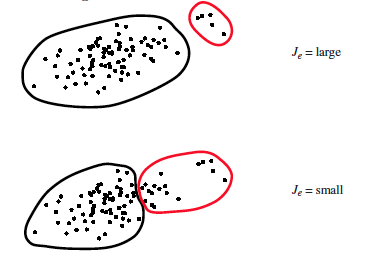
\includegraphics[scale=0.4]{images/je.png}
    \end{center}
    \end{column}    
    
  \end{columns}

\end{frame}

% ============================================== %

\begin{frame}{Обобщение квадратичной ошибки}

Критерий
\begin{eqnarray*}
J_E &=& \sum_{k=1}^K \sum_{\mathbf{x}_i \in C_k} \| \mathbf{x}_i - \mathbf{m}_k \|^2 = \\
&=& \frac 1 2 \sum_{k=1}^K n_k \left[ \frac{1}{n_k^2} \sum_{\mathbf{x}_i \in C_k} \sum_{\mathbf{x}_j \in C_k} \| \mathbf{x}_i - \mathbf{x}_j \|^2 \right] = \\
&=& \frac 1 2 \sum_{k=1}^K n_k \left[ \frac{1}{n_k^2} \sum_{\mathbf{x}_i \in C_k} \sum_{\mathbf{x}_j \in C_k} s(\mathbf{x}_i, \mathbf{x}_j) \right] = \frac 1 2 \sum_{k=1}^K n_k \bar s_k
\end{eqnarray*}
Примеры $\bar s_i$
\[
\bar s_k = \min_{\mathbf{x}_i, \mathbf{x}_j} s(\mathbf{x}_i, \mathbf{x}_j); \quad \bar s_k = \max_{\mathbf{x}_i, \mathbf{x}_j} s(\mathbf{x}_i, \mathbf{x}_j)\]

\end{frame}

% ============================================== %

\begin{frame}{Матрицы разброса}

Матрица разброса внутри кластеров
\[
S_k = \sum_{\mathbf{x}_i \in C_k} (\mathbf{x}_i - \mathbf{m}_k)(\mathbf{x}_i - \mathbf{m}_k)^\top; \quad S_W = \sum_{k=1}^K S_k
\]
Матрица разброса между кластерами
\[
S_B = \sum_{k=1}^K n_k (\mathbf{m}_k - \mathbf{m})(\mathbf{m}_k - \mathbf{m})^\top
\]
Матрица разброса
\[
S_T = \sum_{\mathbf{x}_i \in \mathbf{X}} (\mathbf{x}_i - \mathbf{m})(\mathbf{x}_i - \mathbf{m})^\top
\]
\[
\boxed{S_T = S_W + S_B}
\]

\end{frame}

% ============================================== %

\begin{frame}{Критерии}

\begin{itemize}
\item След
\[
J_E = \text{tr} S_W = \sum_{k=1}^K \sum_{\mathbf{x}_i \in C_K} \| \mathbf{x}_i - \mathbf{m}_k \|^2 \rightarrow \min
\]
\item Детерминант (инвариант относительно растяжения)
\[
J_d = \det S_W \rightarrow \min
\]
\item Инварианты отностиельно линейных преобразований \\ 
\[
J_l = \text{tr} S_W^{-1} S_B = \sum_{j=1}^d \lambda_j \rightarrow \max, \quad J_f = \sum_{j=1}^d \frac{1}{1 + \lambda_j} \rightarrow \min
\]
$\lambda_1, \ldots, \lambda_d$ -- собственные числа $S_W^{-1} S_B$
\end{itemize}

\end{frame}

% ============================================== %

\begin{frame}{Итеративный алгоритм}

Критерий
\[
J_k = \sum_{\mathbf{x}_i \in C_k} \| \mathbf{x}_i - \mathbf{m}_k \|^2, \quad
		\mathbf{m}_k = \frac{1}{n_k} \sum_{\mathbf{x}_i \in C_k} \mathbf{x}_i
\]
Переносим $\hat{\mathbf{x}}$ из кластера $l$ в кластер $k$ 
\[
\mathbf{m}_k^* = \mathbf{m}_k + \frac{\hat{\mathbf{x}} - \mathbf{m}_k}{n_k + 1}, \quad
J_k^* = J_k + \frac{n_k}{n_k+1} \|\hat{\mathbf{x}} - \mathbf{m}_k \|^2
\]
\[
\mathbf{m}_l^* = \mathbf{m}_l - \frac{\hat{\mathbf{x}} - \mathbf{m}_l}{n_l - 1}, \quad
J_l^* = J_l - \frac{n_l}{n_l - 1} \|\hat{\mathbf{x}} - \mathbf{m}_l \|^2
\]
Перенос имеет смысл, если
\[
\frac{n_l}{n_l - 1} \|\hat{\mathbf{x}} - \mathbf{m}_l \|^2 > \frac{n_k}{n_k+1} \|\hat{\mathbf{x}} - \mathbf{m}_k \|^2
\]

\end{frame}

% ============================================== %

\begin{frame}{Итеративный алгоритм}

\texttt{cluster($X$, $K$):}

\texttt{\quad инициализируем $C_1, \ldots, C_K$, $n_1, \ldots, n_K$}

\texttt{\quad do:}

\texttt{\quad\quad случайно выбираем $\hat{\mathbf{x}} \in X$}

\texttt{\quad\quad if $n_l > 1$:}

\texttt{\quad\quad\quad $k^* = \arg \min_k J^*$}

\texttt{\quad\quad\quad перемещаем $\hat{\mathbf{x}}$ в $k^*$}

\texttt{\quad until кластеры стабильны или превышено число итераций}

\vspace{1em}
\begin{itemize}
\item[+] Обучение online
\item[---] Локальная оптимизация
\item[---] Зависимость от порядка рассмотрения $\mathbf{x}$
\end{itemize}

\end{frame}

% ============================================== %

\begin{frame}{Качество кластеризации}

\begin{block}{Задача}
Пусть дана обучающая выборка, для которой правильная кластеризация $C$ известна. С помощью выбранного алгоритма получена кластеризация $K$. Проверить, насколько $K$ совпадает с $C$.
\end{block}

\begin{itemize}
\item Rand Index \\
{\it \small
$a$ -- кол-во пар объектов, попавших в один кластер и в $C$, и в $K$ \\
$b$ -- кол-во пар объектов, попавших в разные кластеры и в $C$, и в $K$
\[
RI = \frac{a+b}{C^N_2}
\]
}
\item Mutual Information \\
{\it \small
\[
MI = \sum_{c \in C} \sum_{k \in K} p(c, k) \log \frac{p(c, k)}{p(k)p(c)}
\]
}
\end{itemize}


\end{frame}

% ============================================== %

\begin{frame}{Зоопарк алгоритмов}

По способу формирования кластеров
\begin{itemize}
\item иерархические (hierarchical, agglomerative)
\item поточечные (point assignment)
\end{itemize}

По типу пространства $\mathbf{X}$
\begin{itemize}
\item $\mathbf{X}$ -- евклидово
\item $\mathbf{X}$ -- не евклидово
\end{itemize}

По требованиям к памяти
\begin{itemize}
\item обучающая выборка должна помещаться в основную память
\item поддерживает обработку данных кусками
\end{itemize}

\end{frame}

% ============================================== %

\begin{frame}{Задача модуля}

Классифицировать пользователей социальных сетей с использованием реализованных в ДЗ алгоритмов классификации и регрессии

\vspace{1em}
Презентация 12.04.2014
\begin{enumerate}
\item Описание задачи (1-2 слайда)
	\begin{enumerate}
	\item Количество объектов в выборке
	\item Распределение целевой переменной
	\item Метод тестирования алгоритмов
	\end{enumerate}
\item Каждый участник группы представляет алгоритм (1-2 слайда)
	\begin{enumerate}
	\item Использованные признаки: распределения, преобразования
	\item Алгоритм: реализация и выбор параметров
	\item Метрики качества: результаты
	\end{enumerate}
\item Итоговый выбор (1-2 слайда)
	\begin{enumerate}
	\item Какой выбран алгоритм
	\item Труднсти
	\end{enumerate}
\end{enumerate}
Итог: 6-12 слайдов на группу, 15 мин на доклад, 30 (20 + 10) баллов

\end{frame}

% ============================================== %

\begin{frame}{ДЗ}

Использование готового алгорима = половина баллов (если не оговорено обратное)

\vspace{1em}
Общие замечания
\begin{enumerate}
\item Дедлайны
\item Интерфейс классификаторов: fit/predict/predict\_proba
\end{enumerate}

Пожелания
\begin{enumerate}
\item PEP-8
\item Коменты
\item Адекватный текст коммитов
\end{enumerate}

Обсуждение
\begin{enumerate}
\item Процедура сабмита ДЗ
\item Размер группы
\end{enumerate}

\end{frame}

% ============================================== %

\begin{frame}{Практика: итеративный алгоритм}

\begin{enumerate}
\item Скачать ветку \texttt{clust} из репозитория и убедиться, что все работает
\item Проверить, что предложенный алгоритм кластеризации не является глобальным
\item Реализовать n-restart алгоритма для обеспечения глобальности
\item Поэкспериментировать с раздичными линейными преобразованиями пространства
\item (*) Реализовать критерий оптимальности, инвариантный относительно преобразований
\end{enumerate}

\end{frame}

\end{document}